\documentclass[12pt,letterpaper]{book}

%Colocando paquetes
\usepackage[left=2cm,right=2cm,top=2cm,bottom=2cm]{geometry}
\usepackage[T1]{fontenc}
\usepackage[utf8]{inputenc}
\usepackage[spanish,es-tabla]{babel}
\parindent=0cm %Configurar sangría
\usepackage{amsmath}
\usepackage{amssymb}
\usepackage{amsfonts,latexsym,cancel}
\usepackage{array}
%\usepackage{bm}
\usepackage{float} %Imágenes
\usepackage{fancyhdr} %Cortar formato al documento
\usepackage{graphicx} %Para gráficas
\usepackage{longtable} %Para tablas largas
\usepackage{multicol} %Varias columnas al doc
\usepackage{subfigure} %Varias figuras
\usepackage{anyfontsize}
%\usepackage{hyperref}
\usepackage[colorlinks = true, linkcolor = black, citecolor = black,urlcolor = blue]{hyperref}
%\usepackage{makeidx}







%\includegraphics[scale=•]{•}

\author{Sergio Hernández Sánchez}
\title{Diseño de un Vehiculo Última Milla para uso en paquetería: Aplicación de un sistema AGV}

\date{10 de marzo de 2020}

%\makeatletter
%\let\ps@plain\ps@empty
%\makeatother

\pagestyle{fancy}
\fancyfoot[C]{\thepage}
\fancyhead[L]{\scriptsize \empty}
\renewcommand{\headrulewidth}{0pt}

\begin{document}

\frontmatter %Numerar con números romanos
\begin{center}

\includegraphics[scale=1]{Figures/Logo_azul.png}\\
\vspace*{2\baselineskip}

\textbf{\fontsize{16}{0}{\selectfont{UNIVERSIDAD NACIONAL AUTÓNOMA DE MÉXICO}}}
\vspace*{0\baselineskip}

PROGRAMA DE MAESTRÍA Y DOCTORADO EN INGENIERÍA
MECÁNICA – DISEÑO MECÁNICO

\vspace*{4\baselineskip}

\textbf{DISEÑO DE UN VEHÍCULO DE ÚLTIMA MILLA PARA SU USO EN PAQUETERÍA: APLICACIÓN DE UN SUSTEMA AGV}

\vspace*{5\baselineskip}

TESIS

QUE PARA OPTAR POR EL GRADO DE:

MAESTRO EN INGENIERÍA

\vspace*{5\baselineskip}

PRESENTA:

SERGIO HERNÁNDEZ SÁNCHEZ

\vspace*{4\baselineskip}

TUTOR PRINCIPAL

DR. ALEJANDRO C. RAMÍREZ REIVICH

\vspace*{4\baselineskip}
CIUDAD UNIVERSITARIA, CDMX, MARZO 2020

\thispagestyle{empty}

\end{center}

%\chapter*{AGRADECIMIENTOS}

Irán los agredecimientos personales y para el proyecto
%\chapter*{RESUMEN}

JBWHBASDASDASD
\renewcommand{\contentsname}{TABLA DE CONTENIDO}
\tableofcontents
\renewcommand{\headrulewidth}{0.5pt}

\mainmatter %Numerar con números arábigos
%\chapter{DEFINICIÓN DEL PROYECTO}
\section{Introducción}
\section{Antecedentes}
Última Milla y retos que enfrenta la paquetería
\section{Métodología}
Ciclos y funciones y Enfoque
\section{Trabajo previo}
Descripción de las tesis anteriores
\section{Planteamiento del problema}
¿Cuál es la problemática?
\section{Objetivo}
General y particulares
\section{Alcances}
A qué se llegará
\section{Equipo de trabajo}
Por etapas



\fancyhead{} %Eliminar definiciones previas
%\fancyhead[R]{Diseño de un VUM para uso en paquetería: Aplicación de un sistema AGV} 
\fancyhead[R]{\scriptsize \leftmark}
\fancyhead[L]{\scriptsize \empty}
\chapter{CICLO 1. USUARIO}
\section{Reto}
\section{Usuario en contexto}
\subsection{Observaciones}
\subsection{Entrevistas}
\subsection{Organizar y jerarquización de necesidades}
\section{Soluciones actuales (mercado)}
\section{Contexto pasado, presente y futuro}
\subsection{Estadísticas, normas, reglamentos}
\section{Factores críticos, hallazgos}
\subsection{Necesidades seleccionadas}
\chapter{CICLO 2. EXPERIENCIA}
\section{Redefinición del reto}
\section{Necesidad jerarquizada}
\section{Objetivo (propuesta de valor)}
\section{Requerimientos}
\section{Escenarios}
\section{Personajes}
\section{Mapa de ruta}
\section{Diseño de experiencias}
\section{Nuevas tecnologías}
\section{Factores críticos, hallazgos}
\chapter{CICLO 3. PRODUCTO}
\section{Redefinición del reto}
\section{Principios de diseño}
\section{Requerimientos y especificaciones}
\section{Generación de conceptos}
\section{Evaluación de conceptos}
\section{Selección de concepto}
\section{Construcción de un simulador*}
\section{Resultado de las pruebas}
\section{Aprendizajes y hallazgos}

\chapter{CICLO 4. PROTOTIPO}

\section{Redefinición del reto}

Se plantea que al VUM se le añadan tecnologías que permitan eficientar el proceso de entrega de paquetería, una primera iteración puede ser la aplicación de un sistema AGV (\textit{Automatic Guided Vehicle}, por sus siglas en inglés). Esto con la idea de tener un primer acercamiento con tecnologías revolucionarias que hoy en día se están desarrollando, como lo son los vehículos autónomos.

\section{Problemática}

Retomando algunas de las necesidades obtenidas de nuestros usuarios, nos dimos cuenta que derivan de situaciones culturales del escenario y contexto mismos. Siendo nuestro usuario principal en este ciclo, el cliente, que como se enunció anteriormente es la dueña de la empresa Re!, quien enució algunas de las problemáticas siguientes:

\begin{itemize}
\item Los empleados no pueden acceder con mochilas ni a la bodega ni a la camioneta porque se pueden robar los paquetes.

\item Hacen mal uso del combustible del vehículo, ya sea porque se desvían de la ruta por intereses personales o porque cargan menos cantidad de éste, mientras que reportan haber comprado una mayor cantidad.

\item En la solución planteada, si dicho VUM tiene una velocidad mayor que una bicicleta, puede ser peligroso para ellos mismos, ya que no tenderán a ir siempre rápido, propiciando accidentes.

\item No es conveniente que el VUM tenga piezas que se quiten, ya que los mismos empleados podrían robárselas.

\item En la solución presentada en el capítulo de \textit{experiencia}, cuya solución implica llevar únicamente a los vehículos a un punto intermedio de las zonas de entrega, esto podría generar problemas en la logística, ya que los conductores tendrían que llegar a los puntos de de descarga de los vehículos, dificultando su acceso por cuestiones de movilidad.

\end{itemize}
Con estos hallazgos, se hace evidente que el vehículo y el proceso de entrega es altamente mejorable. por lo que se plantea que el una posible solución sea que dicho VUM sea no tripulado pudiendo entregar en un ambiente controlado.

\section{Objetivo}

Mejorar la eficiencia del sistema de entrega VUM, planteando la implementación de un sistema de Vehículo de Guiado Automático (AGV) en rutas controladas.
%\cite{yo}

\section{Productos en desarrollo}

Algunos de los conceptos que se han ido desarrollando en los últimos años se presentaron en la sección 1.4, cuyo nombre es \textit{contexto pasado, presente futuro}. Si bien en este se presentan propuestas de vehículos de reparto tripulados de dos y tres ruedas, también se presentan algunos que se proyectaban como conceptos de solución no tripulada, como drones y robots. \\
En esta seción presentaremos más en específico que se ha hecho en el ámbito de la róbotica para reparto.

\subsection{Starship} 
Esta empresa fue creada en 2014 y sólo cautro años implementó su negocio de entrega de comida y paquetería por medio de un robot móvil autónomo de seis ruedas en la universidad de Milton Keynes, en Reino Unido. Este es navega por las banquetas, detecta obstáculos, personas y demás imprevistos que se presenten en su recorrido. A la fecha se realiza entregas en otras universidades, acumulando más de 100,000 entregas \cite{starship}.
	\begin{figure}[hbtp]

	\centering
	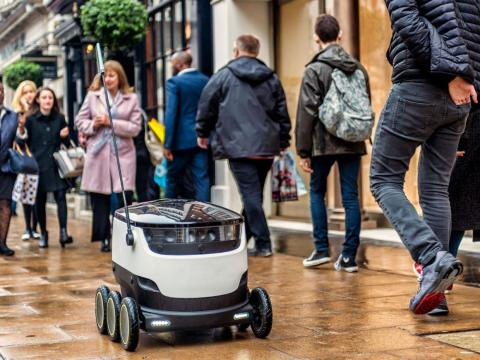
\includegraphics[scale=0.6]{Figures/Starship_Picture.jpg}
	\caption{Robot autónomo de Starship\cite{starship_picture}.} 
	\end{figure}

Algunas de las características de este robot son las siguientes \cite{starship_feature}:

\begin{itemize}
\item Sensores: Ultrasónico, camera de tiempo de vuelo (ToF camera), cámara estereo.

\item Características importantes: Utilizando dichos sensores e inteligencia artificial, puede mapear y entender el entorno, permitiéndole detectar objetos y saber su ubicación.

\item Dimensiones: 55.9 cm de altura, 68.9 cm de largo y 55.9 cm de ancho.

\item Peso: 20 kg.

\item Velocidad: 6 km/h.

\item Seguridad: El compartimento de carga está bloqueado, solo se puede abrir con la aplicación del teléfono inteligente del receptor. Además, el robot tiene seguimiento de su ubicación por parte de la empresa y del usuario, al llegar al destino, le enviará una notificación \cite{starship}.
\end{itemize}







\subsection{Por definir}
\begin{itemize}
\item Sistema para que no se caiga
\item Actuación

\begin{itemize}
\item Aceleración
\item Dirección
\item Frenado
\item Luces
\end{itemize}

Sensado
\begin{itemize}
\item Detección de obstáculos
\item Detección de ruta
\item Conocer el estado del VEnTUM
\end{itemize}

Procesamiento (Programación para las diferentes condiciones de funcionamiento)

\end{itemize}




\section{GENERAR. Generación de conceptos}
Generación de conceptos y selección
\section{GENERAR. Selección de conceptos}
\section{GENERAR. Desarrollo de la propuesta}
\section{PROBAR. Simuladores, maquetas, prototipos}

\section{APRENDER. Análisis de hallazgos}


%\include{Section_thesis/Conclutions}
%\chapter*{TRABAJO A FUTURO}




\end{document}